% ==========================================================
% Slides de apresentação do SIGEJ (Commit Júnior)
% Compilar a partir da raiz do repositório:
%   latexmk -pdf -outdir=build slide.tex   (ou pdflatex slide.tex, 2x)
% ==========================================================
\documentclass[aspectratio=169,9pt]{beamer}

\usepackage[utf8]{inputenc}
\usepackage[T1]{fontenc}
\usepackage[brazil]{babel}
\usepackage{lmodern}
\usepackage{graphicx}
\usepackage{booktabs}
\usepackage{array}
\newcolumntype{P}[1]{>{\raggedright\arraybackslash}p{#1}}
\usepackage{tikz}
\usetikzlibrary{arrows.meta,positioning}

% imagens: raiz, Telas/ e fig/ (mesmas pastas da monografia)
\graphicspath{{./}{Telas/}{fig/}}

% ---------- tema ----------
\usetheme{Madrid}
\definecolor{cefet}{RGB}{23,58,102}
\definecolor{destaque}{RGB}{200,60,40}
\setbeamercolor{structure}{fg=cefet}
\setbeamercolor{palette primary}{bg=cefet,fg=white}
\setbeamercolor{palette secondary}{bg=cefet!85!black,fg=white}
\setbeamercolor{palette tertiary}{bg=cefet!70!black,fg=white}
\setbeamercolor{frametitle}{bg=cefet,fg=white}
\setbeamerfont{frametitle}{size=\large}
\setbeamertemplate{navigation symbols}{}
\setbeamertemplate{footline}{%
  \leavevmode\hbox{%
    \begin{beamercolorbox}[wd=.85\paperwidth,ht=2.4ex,dp=1ex,left,leftskip=2mm]{palette tertiary}
      \scriptsize SIGEJ -- Commit Júnior\hfill
    \end{beamercolorbox}%
    \begin{beamercolorbox}[wd=.15\paperwidth,ht=2.4ex,dp=1ex,right,rightskip=2mm]{palette tertiary}
      \scriptsize\insertframenumber{} / \inserttotalframenumber
    \end{beamercolorbox}}%
}
\setbeamertemplate{itemize items}[circle]
\setlength{\leftmargini}{1.1em}

% ---------- helpers de diagrama de classes ----------
\tikzset{
  cls/.style={draw=cefet, fill=cefet!8, rounded corners=1pt, font=\footnotesize\bfseries,
              inner sep=3pt, minimum height=0.6cm, align=center},
  ref/.style={cls, dashed, fill=white, text=black!70},
  lbl/.style={font=\scriptsize\itshape, fill=white, inner sep=1pt},
  mlt/.style={font=\scriptsize, inner sep=1.2pt},
  comp/.style={{Diamond[length=6pt,width=4.5pt]}-},
  agg/.style={{Diamond[open,length=6pt,width=4.5pt]}-},
  nav/.style={-{Straight Barb[length=4pt,width=5pt]}},
}
\newcommand{\cls}[3]{\node[cls] (#1) at (#2) {#3};}
\newcommand{\refcls}[3]{\node[ref] (#1) at (#2) {#3};}
% \assoc[estilo]{origem}{destino}{rótulo}{mult. origem}{mult. destino}
\newcommand{\assoc}[6][]{%
  \draw[#1] (#2) to node[lbl,midway]{#4} node[mlt,pos=.13,auto]{#5} node[mlt,pos=.87,auto]{#6} (#3);}

% leitura das associações
\newenvironment{leitura}{%
  \par\footnotesize\textbf{\color{cefet}Leitura das associações (nos dois sentidos)}\par\vspace{2pt}
  \begin{itemize}\setlength{\itemsep}{3pt}\setlength{\parsep}{0pt}\footnotesize}%
  {\end{itemize}}

\title[SIGEJ]{SIGEJ -- Sistema Integrado de Gestão de Empresa Júnior}
\subtitle{Modelagem do sistema da Commit Júnior}
\author[Luan Lana Maia \& Yuri Espindola]{Luan Lana Maia \and Yuri Espindola}
\institute[CEFET-MG Timóteo]{%
  CEFET-MG -- Campus Timóteo\\
  Engenharia de Computação -- Laboratório de Modelagem de Sistemas\\
  Orientação: Profa.\ Márcia Valéria}
\date{\today}

\begin{document}

% ==========================================================
\begin{frame}[plain]
  \titlepage
\end{frame}

% ==========================================================
\begin{frame}{Roteiro da apresentação}
  \begin{columns}[T]
    \begin{column}{.58\textwidth}
      \begin{enumerate}\setlength{\itemsep}{5pt}
        \item \textbf{Contexto}: sistema, motivação e diferencial
        \item \textbf{Diagrama de Casos de Uso} (DCU)
        \item \textbf{Regras de Negócio}
        \item \textbf{Requisitos Não Funcionais}
        \item \textbf{Projeto de Interface e Interação}
        \item \textbf{Diagrama de Classes}
        \item \textbf{Perguntas e considerações}
      \end{enumerate}
    \end{column}
    \begin{column}{.38\textwidth}
      \vspace{4pt}
      \begin{block}{Foco}
        Apresentar a \textbf{modelagem} do sistema: o que ele faz, para quem, com quais regras e como os dados se organizam.
      \end{block}
    \end{column}
  \end{columns}
\end{frame}

% ==========================================================
\section{Contexto}
\begin{frame}{Contexto: a Commit Júnior}
  \begin{columns}[T]
    \begin{column}{.60\textwidth}
      \begin{itemize}\setlength{\itemsep}{4pt}
        \item \textbf{Empresa Júnior} sem fins lucrativos, gerida por estudantes de graduação do CEFET-MG; oferece consultoria e soluções computacionais.
        \item Concebida em 2018--2019 por estudantes de Administração e Computação; federada ao MEJ em 2020.
        \item Atua nos campi \textbf{Belo Horizonte} e \textbf{Timóteo}.
        \item \textbf{Departamentos:} Projetos (Automação e WordPress), Gestão \& Gente (Jurídico e Pessoas), Financeiro, Comercial e Marketing.
        \item Rotatividade alta: mandatos curtos e trocas frequentes de gestão.
      \end{itemize}
    \end{column}
    \begin{column}{.36\textwidth}
      \centering\scriptsize\textbf{Hierarquia (4 níveis)}\\[4pt]
      \begin{tikzpicture}[node distance=0.35cm, every node/.style={font=\scriptsize, align=center}]
        \node[draw=cefet, fill=cefet!25, minimum width=4.4cm, minimum height=0.7cm] (a) {Diretoria Executiva\\{\tiny Presidente e Diretores}};
        \node[draw=cefet, fill=cefet!16, minimum width=4.4cm, minimum height=0.7cm, below=of a] (b) {Gerentes\\{\tiny nível tático}};
        \node[draw=cefet, fill=cefet!9, minimum width=4.4cm, minimum height=0.7cm, below=of b] (c) {Membros efetivos\\{\tiny nível operacional}};
        \node[draw=cefet, fill=cefet!4, minimum width=4.4cm, minimum height=0.7cm, below=of c] (d) {Trainees\\{\tiny em capacitação}};
        \draw[-{Stealth}] (a) -- (b); \draw[-{Stealth}] (b) -- (c); \draw[-{Stealth}] (c) -- (d);
      \end{tikzpicture}
    \end{column}
  \end{columns}
\end{frame}

% ==========================================================
\begin{frame}{Contexto: como é feito hoje}
  \small
  \renewcommand{\arraystretch}{1.25}
  \begin{tabular}{@{}>{\bfseries}P{2.6cm}P{5.8cm}P{4.2cm}@{}}
    \toprule
    Frente & Como é hoje & Problema \\
    \midrule
    Cadastro e termos & Google Forms $\rightarrow$ Google Sheets $\rightarrow$ termos gerados à mão $\rightarrow$ Autentique & Retrabalho, campos em branco, ex-membros ainda ``ativos'' \\
    Horas de extensão & Planilha; cálculo manual pelo assessor da presidência; envio por WhatsApp ao professor, que lança no SIGAA & Erros de contagem e digitação; atrasos na formalização \\
    Pontos disciplinares & Painel no Notion; validade e reincidência conferidas visualmente & Sem automação; qualquer integrante pode editar \\
    Diretório e agenda & Quadros no Notion; RG e 1-on-1 por mensagens e calendários pessoais & Dados desatualizados e choques de horário \\
    Governança & Decisões na Diretoria Executiva; privilégios concentrados em contas individuais & Risco a cada troca de gestão \\
    \bottomrule
  \end{tabular}
\end{frame}

% ==========================================================
\begin{frame}{Contexto: motivação e diferencial}
  \begin{columns}[T]
    \begin{column}{.38\textwidth}
      \begin{block}{Sistema}
        Plataforma \textbf{web} integrada para a gestão da Commit Júnior: membros e termos, horas de extensão, disciplina, diretório, avisos, calendário, projetos, comercial, financeiro e governança.
      \end{block}
      \begin{block}{Motivação}
        Substituir planilhas, Notion e WhatsApp por um sistema com \textbf{integridade}, \textbf{rastreabilidade}, proteção de dados sensíveis e menos tarefas manuais.
      \end{block}
    \end{column}
    \begin{column}{.58\textwidth}
      \textbf{\color{cefet}Diferencial}
      \begin{itemize}\setlength{\itemsep}{3pt}\small
        \item \textbf{Sem conta de administrador:} ações críticas viram proposta e são votadas pela diretoria.
        \item Cadastro \textbf{centralizado}, com histórico preservado (desativação lógica).
        \item \textbf{Horas de extensão} e tempo de empresa calculados automaticamente; relatório por e-mail ao professor orientador.
        \item Penalidades com \textbf{expiração automática}, agravante por reincidência e contestação formal.
        \item Diretório só com membros ativos; \textbf{calendário único} sem choque de horário.
        \item Integração com \textbf{Autentique}, \textbf{GitHub} e SMTP institucional.
      \end{itemize}
    \end{column}
  \end{columns}
\end{frame}

% ==========================================================
\section{DCU}
\begin{frame}[plain]
  \centering
  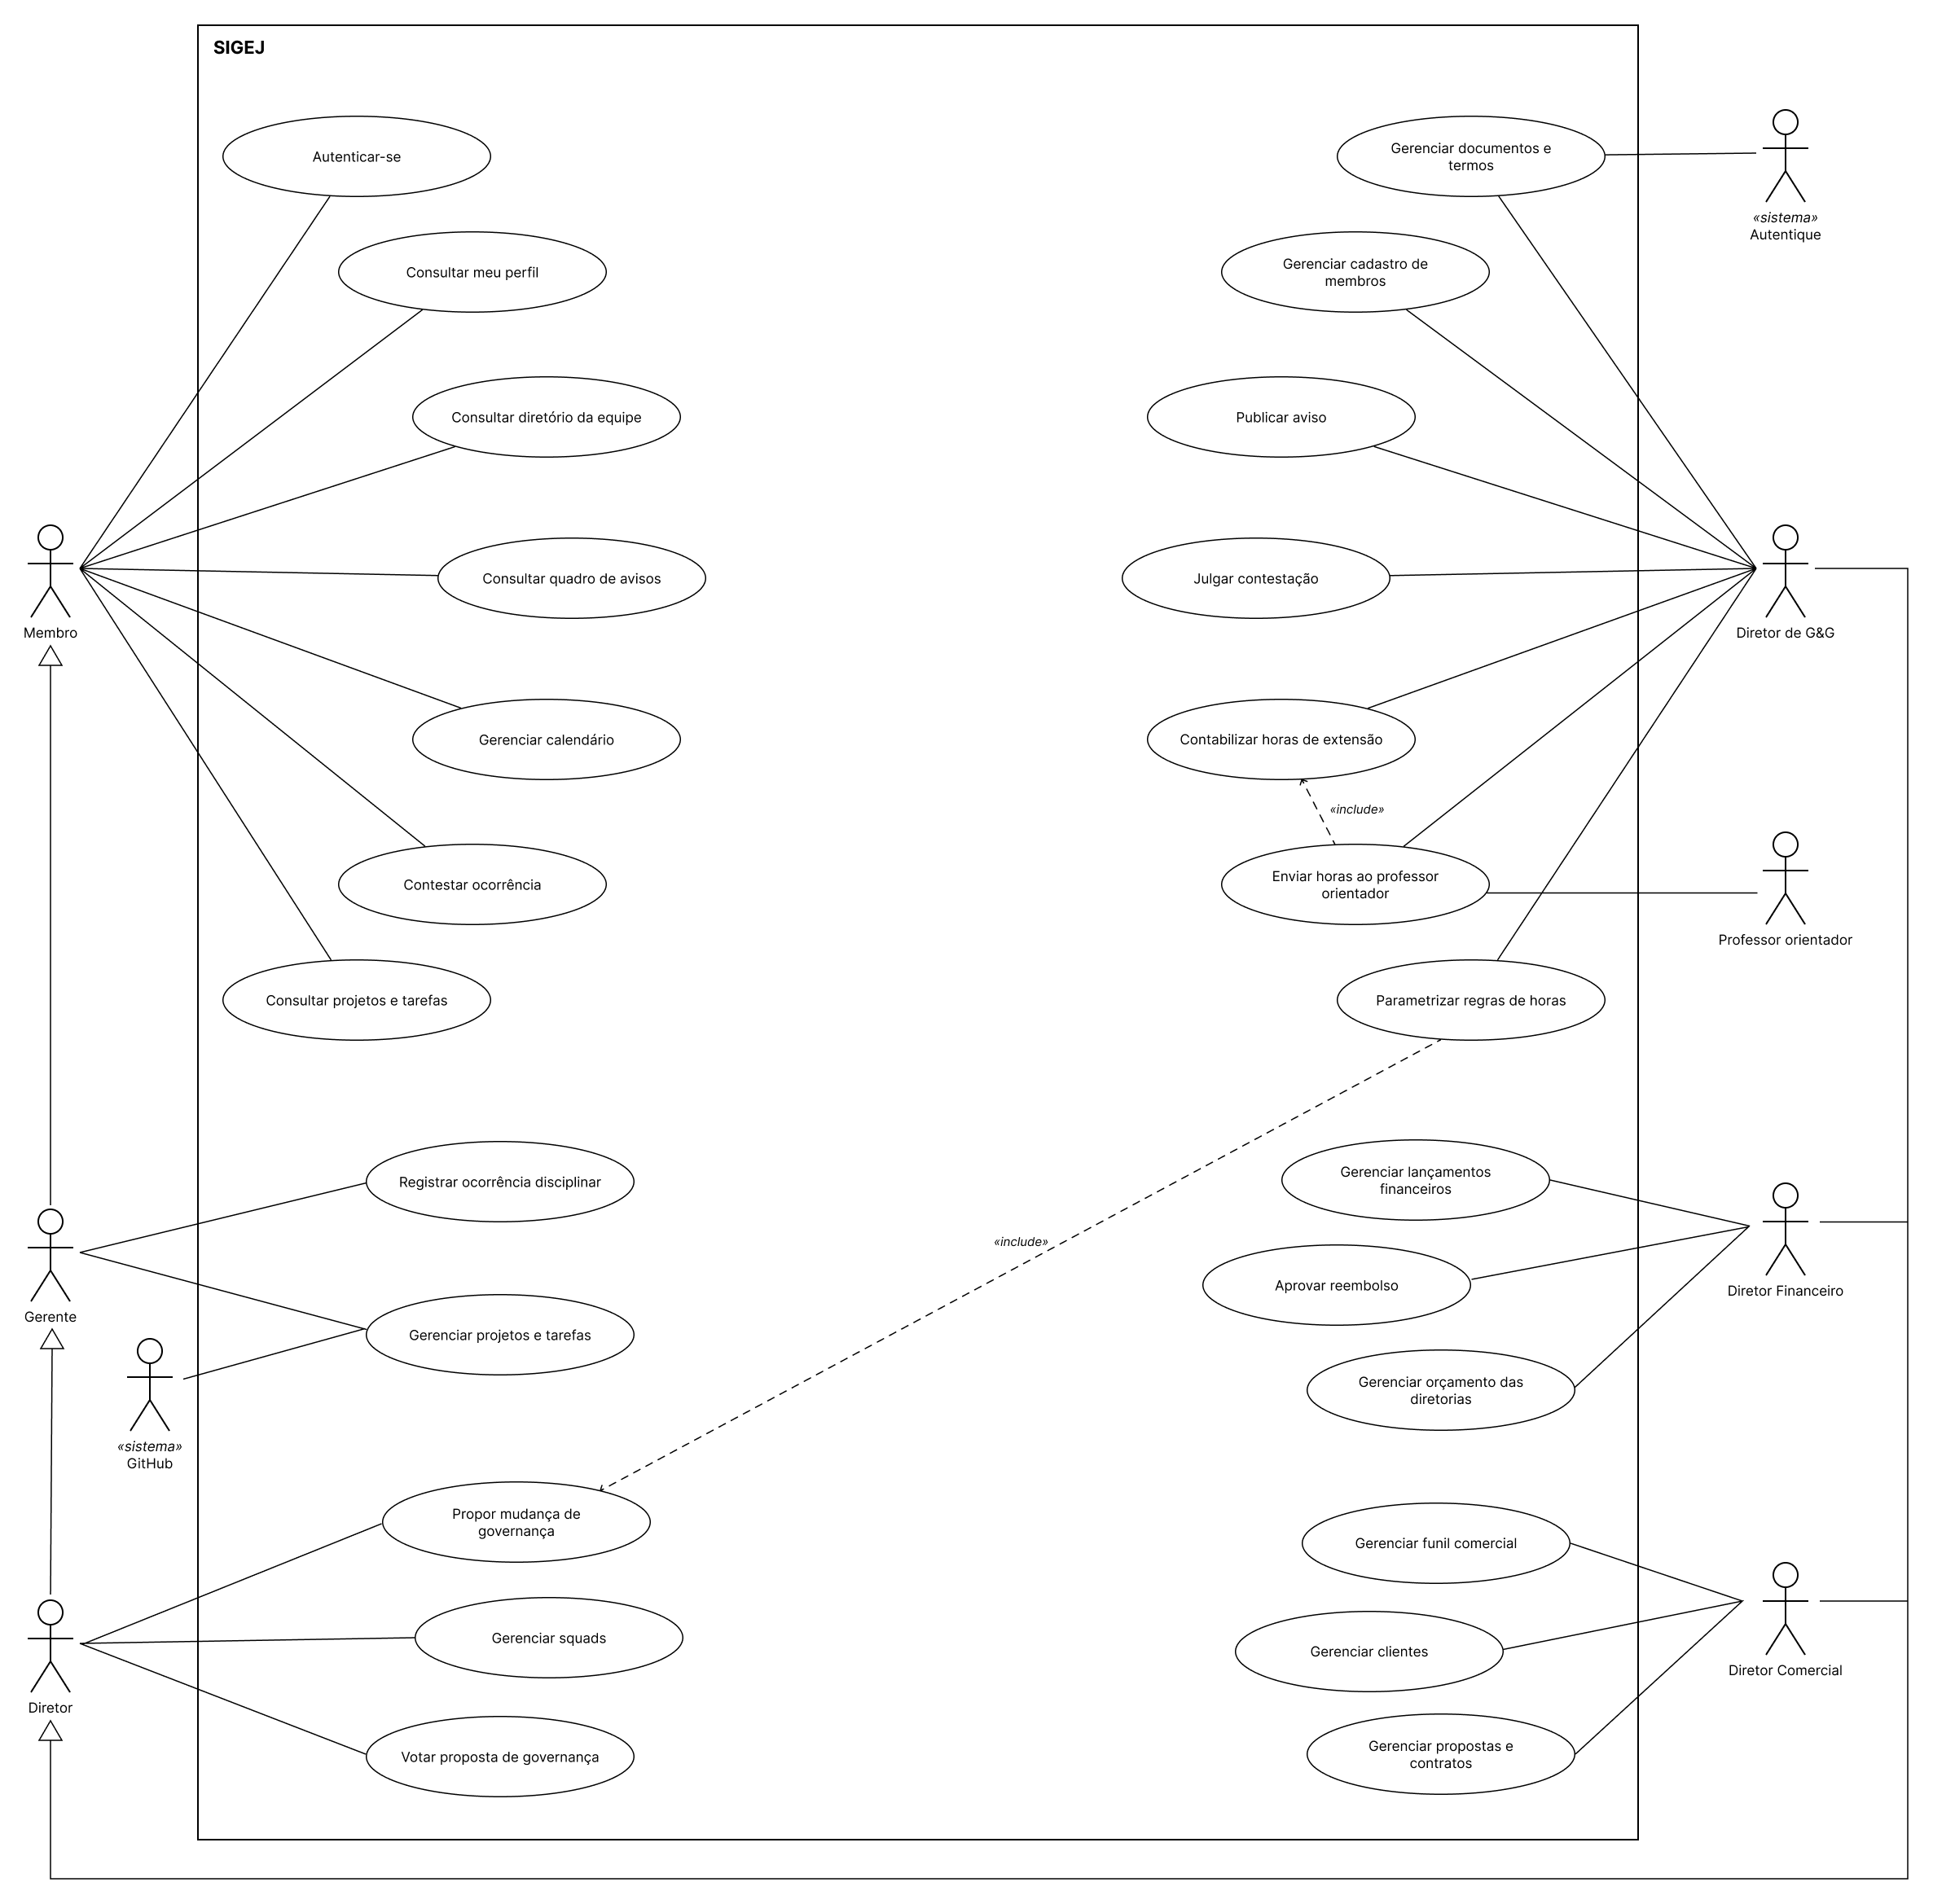
\includegraphics[height=\paperheight,keepaspectratio]{diagrama.png}
\end{frame}

\begin{frame}{DCU: atores e casos de uso}
  \footnotesize
  \begin{columns}[T]
    \begin{column}{.325\textwidth}
      \textbf{\color{cefet}Membro}
      \begin{itemize}\setlength{\itemsep}{0pt}
        \item UC-01 Autenticar-se
        \item UC-02 Consultar meu perfil
        \item UC-03 Consultar diretório da equipe
        \item UC-04 Consultar quadro de avisos
        \item UC-05 Gerenciar calendário
        \item UC-06 Contestar ocorrência
        \item UC-07 Consultar projetos e tarefas
      \end{itemize}
      \vspace{3pt}
      \textbf{\color{cefet}Gerente} {\tiny(especializa Membro)}
      \begin{itemize}\setlength{\itemsep}{0pt}
        \item UC-15 Registrar ocorrência disciplinar
        \item UC-17 Gerenciar projetos e tarefas {\tiny(GitHub)}
      \end{itemize}
      \vspace{3pt}
      \textbf{\color{cefet}Diretor} {\tiny(especializa Gerente)}
      \begin{itemize}\setlength{\itemsep}{0pt}
        \item UC-18 Propor mudança de governança
        \item UC-19 Votar proposta de governança
        \item UC-25 Gerenciar squads
      \end{itemize}
    \end{column}
    \begin{column}{.34\textwidth}
      \textbf{\color{cefet}Diretor de G\&G}
      \begin{itemize}\setlength{\itemsep}{0pt}
        \item UC-08 Gerenciar documentos e termos {\tiny(Autentique)}
        \item UC-09 Gerenciar cadastro de membros
        \item UC-10 Publicar aviso
        \item UC-11 Julgar contestação
        \item UC-12 Parametrizar regras de horas
        \item UC-13 Contabilizar horas de extensão
        \item UC-14 Enviar horas ao professor orientador {\tiny(inclui UC-13)}
      \end{itemize}
    \end{column}
    \begin{column}{.31\textwidth}
      \textbf{\color{cefet}Diretor Financeiro}
      \begin{itemize}\setlength{\itemsep}{0pt}
        \item UC-20 Gerenciar lançamentos financeiros
        \item UC-21 Aprovar reembolso
        \item UC-22 Gerenciar orçamento das diretorias
      \end{itemize}
      \vspace{3pt}
      \textbf{\color{cefet}Diretor Comercial}
      \begin{itemize}\setlength{\itemsep}{0pt}
        \item UC-16 Gerenciar funil comercial
        \item UC-23 Gerenciar clientes
        \item UC-24 Gerenciar propostas e contratos
      \end{itemize}
      \vspace{3pt}
      \textbf{\color{cefet}Atores externos}
      \begin{itemize}\setlength{\itemsep}{0pt}
        \item Professor orientador (lança no SIGAA)
        \item Autentique (assinatura eletrônica)
        \item GitHub (repositórios)
      \end{itemize}
    \end{column}
  \end{columns}
\end{frame}

% ==========================================================
\section{Regras de Negócio}
\begin{frame}{Regras de Negócio}
  \small
  \renewcommand{\arraystretch}{1.2}
  \begin{tabular}{@{}l>{\bfseries}P{4.6cm}P{7.2cm}@{}}
    \toprule
    \textcolor{cefet}{\textbf{RN01}} & Unicidade cadastral & Identificação única por CPF e matrícula \\
    \textcolor{cefet}{\textbf{RN02}} & Cômputo proporcional de horas & Tempo no cargo $\times$ taxa horária parametrizada \\
    \textcolor{cefet}{\textbf{RN03}} & Preservação histórica & Sem exclusão física: status ``Desligado'' ou ``Alumnus'' \\
    \textcolor{cefet}{\textbf{RN04}} & Visibilidade a membros ativos & Diretório só com ativos; histórico restrito ao Diretor de G\&G \\
    \textcolor{cefet}{\textbf{RN05}} & Caducidade e agravamento & Toda ocorrência expira; reincidência no prazo aplica agravante \\
    \textcolor{cefet}{\textbf{RN06}} & Incompatibilidade de agendamentos & Bloqueia reunião com participante já comprometido no horário \\
    \textcolor{cefet}{\textbf{RN07}} & Registro de ocorrências & Só Gerentes e Diretores registram; o membro é notificado \\
    \textcolor{cefet}{\textbf{RN08}} & Contestação de ocorrências & Fica ``Pendente'' até o julgamento; só o membro afetado contesta \\
    \textcolor{cefet}{\textbf{RN09}} & Envio de horas & Só para horas já contabilizadas; passam a ``Enviado'' \\
    \textcolor{cefet}{\textbf{RN10}} & Aprovação de reembolsos & Só o Diretor Financeiro; decisão registrada com data e autor \\
    \textcolor{cefet}{\textbf{RN11}} & Votação de governança & Sem administrador; ação crítica exige aprovação de outros 2 diretores \\
    \bottomrule
  \end{tabular}
\end{frame}

% ==========================================================
\section{Requisitos Não Funcionais}
\begin{frame}{Requisitos Não Funcionais}
  \small
  \renewcommand{\arraystretch}{1.3}
  \begin{tabular}{@{}l>{\bfseries}P{4.3cm}P{2.9cm}P{1.9cm}P{3.1cm}@{}}
    \toprule
    & Requisito & Categoria & Prioridade & Em uma linha \\
    \midrule
    \textcolor{cefet}{\textbf{RNF01}} & Portabilidade web & Portabilidade & Essencial & Navegadores modernos, desktop e mobile \\
    \textcolor{cefet}{\textbf{RNF02}} & Desempenho e tempo de resposta & Desempenho & Importante & Listagens em até 2 s \\
    \textcolor{cefet}{\textbf{RNF03}} & Controle de acesso (RBAC) & Segurança & Essencial & Acesso por perfil \\
    \textcolor{cefet}{\textbf{RNF04}} & Criptografia de dados & Segurança & Essencial & Senhas com hash; dados sensíveis cifrados \\
    \textcolor{cefet}{\textbf{RNF05}} & Responsividade e usabilidade & Facilidade de uso & Essencial & Interface adaptável a qualquer tela \\
    \textcolor{cefet}{\textbf{RNF06}} & Auditoria (logs) & Confiabilidade & Importante & Logs imutáveis com data e autor \\
    \textcolor{cefet}{\textbf{RNF07}} & Integração com serviços externos & Interoperabilidade & Importante & Autentique, GitHub e SMTP \\
    \bottomrule
  \end{tabular}
\end{frame}

% ==========================================================
\section{Projeto de Interface e Interação}
\begin{frame}{Projeto de Interface e Interação}
  \begin{columns}[T]
    \begin{column}{.48\textwidth}
      \begin{itemize}\setlength{\itemsep}{4pt}
        \item Protótipo no \textbf{Figma}: \textbf{38 telas} (PT-001 a PT-038), rastreadas aos 25 casos de uso.
        \item Menu lateral por módulo, com as telas organizadas conforme o perfil do usuário.
        \item Ideia central: \textbf{manter o que as pessoas já usam hoje} (tabelas, painéis e cartões do Notion e do Sheets) e acrescentar o que falta: automação, controle de acesso e rastreabilidade.
      \end{itemize}
      \vspace{4pt}
      \href{https://www.figma.com/design/DR6oCNn8QeMXILJPJx4L4D}{\scriptsize\textcolor{cefet}{\underline{Abrir o protótipo no Figma}}}
    \end{column}
    \begin{column}{.48\textwidth}
      \textbf{\color{cefet}6 fluxos principais}
      \begin{enumerate}\footnotesize\setlength{\itemsep}{3pt}
        \item \textbf{Membro e contestação}: login, perfil, penalidades
        \item \textbf{Gestão \& Gente}: cadastro, desligamento, termos, julgamento
        \item \textbf{Horas de extensão}: regras, contabilização, envio
        \item \textbf{Gerente}: ocorrências, projetos e tarefas
        \item \textbf{Comunicação e agenda}: diretório, squads, avisos, calendário
        \item \textbf{Diretoria, comercial e finanças}: votação, funil, contratos, reembolsos
      \end{enumerate}
    \end{column}
  \end{columns}
\end{frame}

% ---------- antes x depois ----------
\newcommand{\antesdepois}[7]{% titulo, imgAntes, legAntes, imgDepois, legDepois, igual, novo
  \begin{frame}{#1}
    \begin{columns}[T]
      \begin{column}{.485\textwidth}
        \centering\footnotesize\textbf{Hoje:} #3\\[2pt]
        \parbox[c][4.0cm][c]{\linewidth}{\centering\fbox{\includegraphics[width=\dimexpr\linewidth-2\fboxsep-2\fboxrule\relax,height=3.8cm,keepaspectratio]{#2}}}
      \end{column}
      \begin{column}{.485\textwidth}
        \centering\footnotesize\textbf{No SIGEJ:} #5\\[2pt]
        \parbox[c][4.0cm][c]{\linewidth}{\centering\fbox{\includegraphics[width=\dimexpr\linewidth-2\fboxsep-2\fboxrule\relax,height=3.8cm,keepaspectratio]{#4}}}
      \end{column}
    \end{columns}
    \vspace{4pt}
    \begin{columns}[T]
      \begin{column}{.485\textwidth}
        \footnotesize\textbf{\color{cefet}O que se mantém}\\ #6
      \end{column}
      \begin{column}{.485\textwidth}
        \footnotesize\textbf{\color{destaque}O que muda (e por quê)}\\ #7
      \end{column}
    \end{columns}
  \end{frame}}

\antesdepois{Interface: cadastro de membros}
  {gerenciamento-de-membros}{planilha no Google Sheets}
  {membros-lista}{PT-004, cadastro de membros}
  {Listagem em tabela com campus, curso, cargo e situação, como na planilha.}
  {Filtros por situação, edição e desligamento com inativação lógica; edição crítica vira proposta de governança. Evita linhas apagadas e dados em branco.}

\antesdepois{Interface: horas de extensão}
  {gerenciamento-de-horas}{planilha de horas no Google Sheets}
  {horas-contabilizacao}{PT-010, contabilização de horas}
  {Tabela por membro com campus, ingresso e horas, como na planilha.}
  {Total calculado pelo histórico de cargos e pelas regras por cargo, com envio por e-mail ao professor. Elimina a conta manual e o WhatsApp.}

\antesdepois{Interface: pontos e penalidades}
  {tela-lancamento-de-pontos}{painel de pontos no Notion}
  {pontos-registrar-ocorrencia}{PT-012, registrar ocorrência}
  {Lançamento de pontos por membro, com cargo e total de pontos.}
  {Infração do catálogo, cálculo automático de pontos, validade e agravante; acesso só para Gerentes e Diretores. Substitui a conferência visual e a edição aberta.}

\antesdepois{Interface: diretório da equipe}
  {tela-notion}{quadro de membros no Notion}
  {diretorio-equipe}{PT-007, diretório da equipe}
  {Consulta por campus, diretoria e squad, com contatos de cada pessoa.}
  {Cartões com horas e engajamento; exibe só membros ativos. Resolve o problema de ex-membros ainda listados.}

\begin{frame}{Onde o sistema é mais complexo que hoje, e por quê}
  \begin{columns}[T]
    \begin{column}{.60\textwidth}
      \scriptsize
      \renewcommand{\arraystretch}{1.35}
      \begin{tabular}{@{}>{\bfseries}P{2.6cm}P{4.9cm}@{}}
        \toprule
        Acréscimo & Por que é necessário \\
        \midrule
        Governança por votação (sem administrador) & Presidência muda muito; nenhuma conta deve concentrar poder \\
        Perfis de acesso (RBAC) & Dados civis e disciplinares são sensíveis \\
        Trilha de auditoria & Hoje o painel de pontos aceita edição sem rastro \\
        Cálculos automáticos & Horas, validade e agravantes deixam de depender de conferência visual \\
        Contestação formal & Dá ao membro um canal para contestar pontos \\
        Integrações & Autentique, SMTP e GitHub substituem cópia manual e WhatsApp \\
        \bottomrule
      \end{tabular}
    \end{column}
    \begin{column}{.36\textwidth}
      \centering\scriptsize\textbf{PT-025: homologar proposta}\\[2pt]
      \fbox{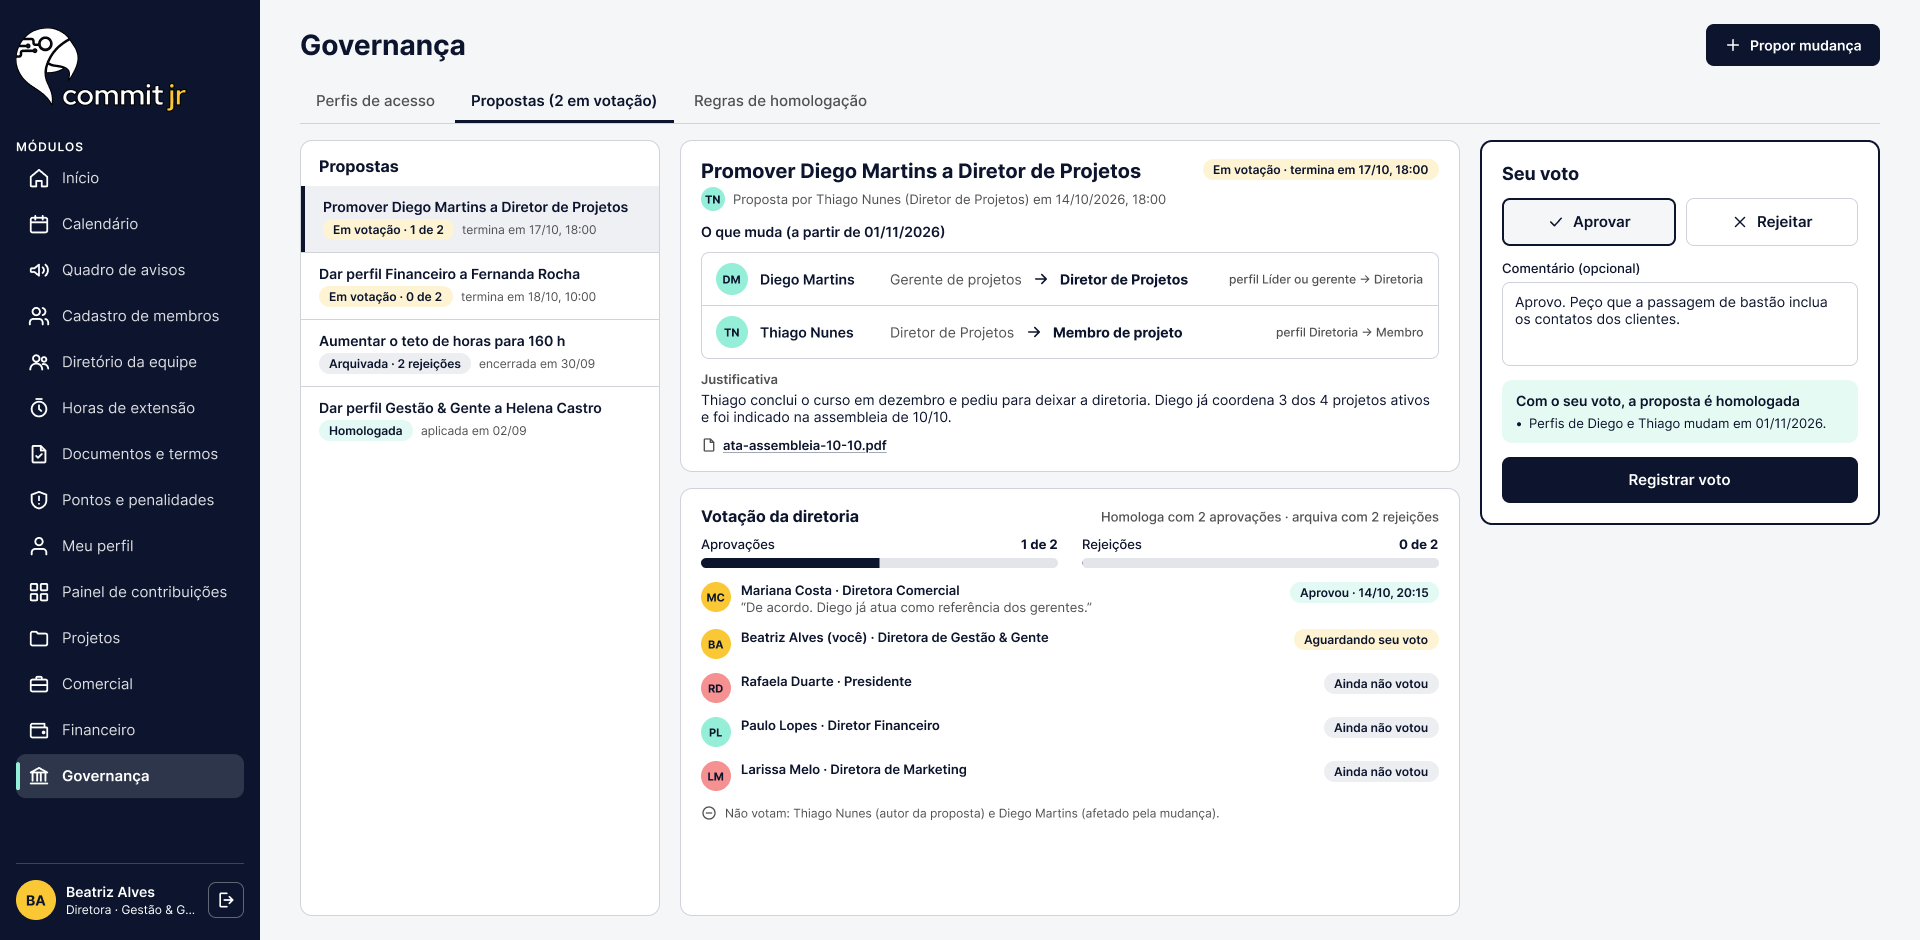
\includegraphics[width=\dimexpr\linewidth-2\fboxsep-2\fboxrule\relax]{governanca-homologar-proposta}}
    \end{column}
  \end{columns}
\end{frame}

% ==========================================================
\section{Diagrama de Classes}
\begin{frame}{Diagrama de Classes: visão geral}
  \begin{columns}[c]
    \begin{column}{.52\textwidth}
      \centering
      \fbox{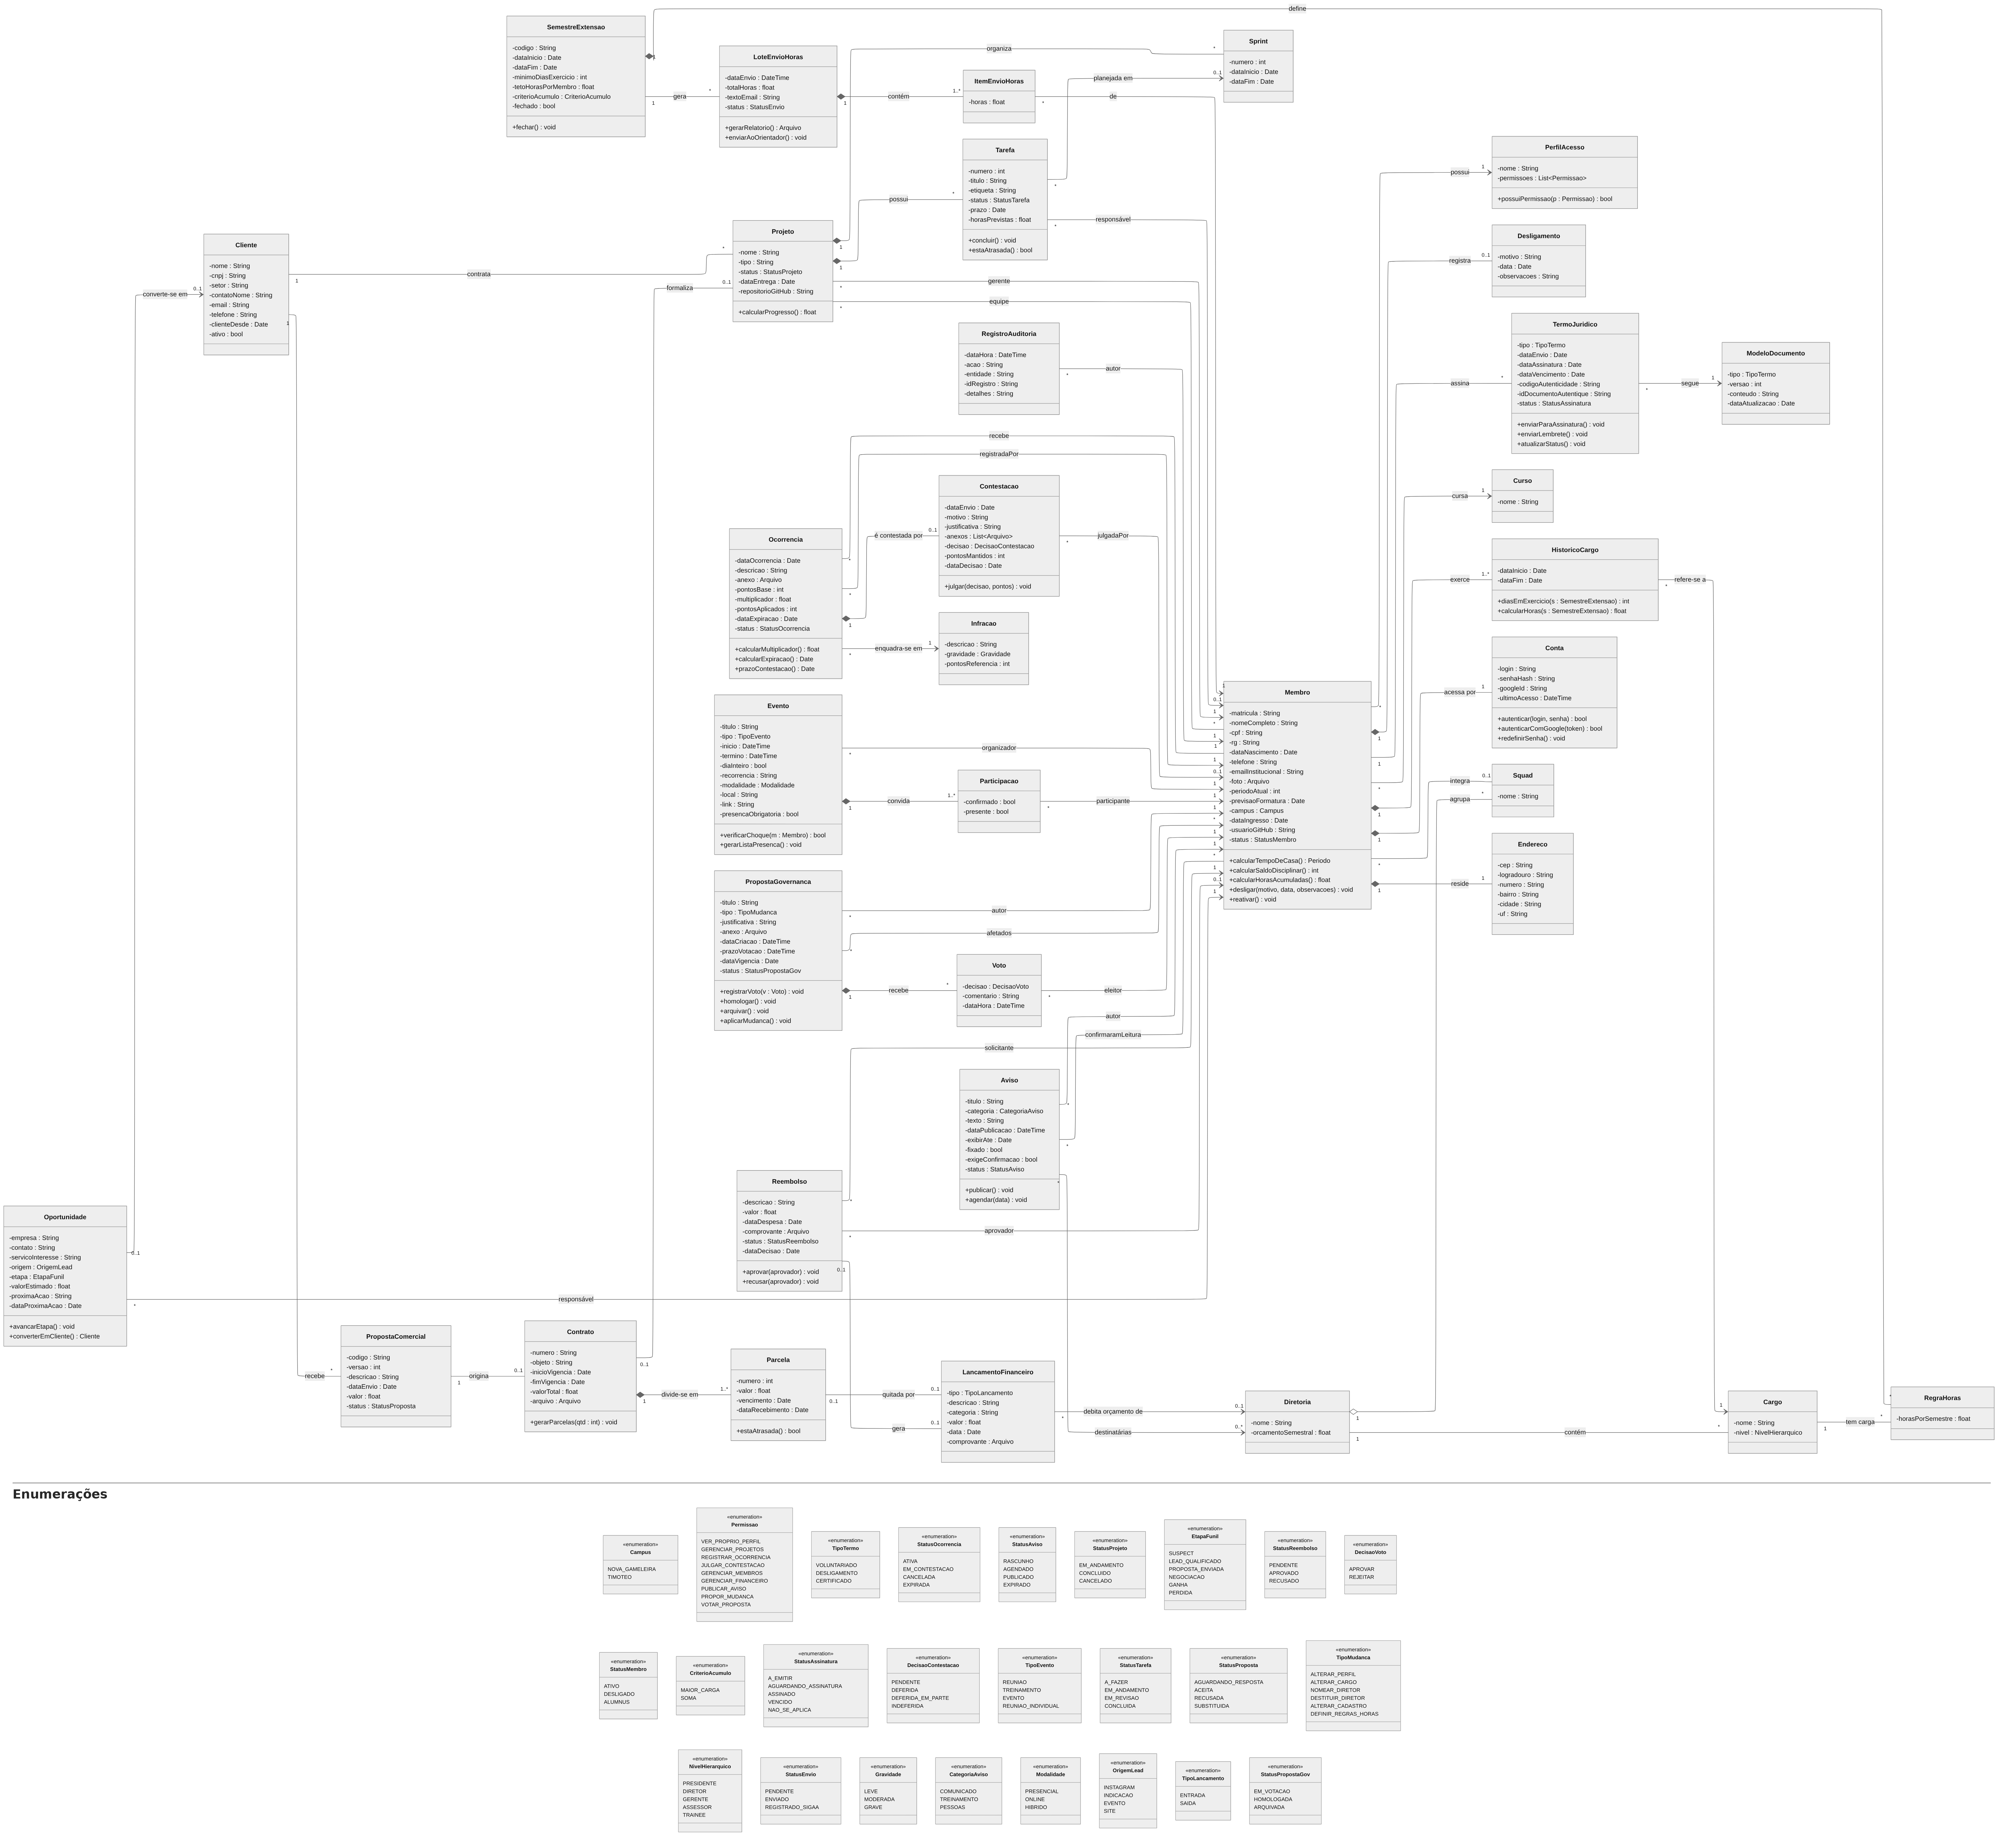
\includegraphics[height=6.1cm,keepaspectratio]{diagrama-classes}}
    \end{column}
    \begin{column}{.44\textwidth}
      \small
      Construído a partir do minimundo, dos casos de uso e dos campos das telas. Organizado em \textbf{módulos}:
      \begin{enumerate}\scriptsize\setlength{\itemsep}{2pt}
        \item Pessoas e acesso
        \item Horas de extensão e documentos
        \item Controle disciplinar
        \item Comunicação e agenda
        \item Projetos
        \item Comercial
        \item Financeiro
        \item Governança e auditoria
      \end{enumerate}
      \vspace{3pt}
      {\scriptsize Nos próximos slides, cada associação é lida nos dois sentidos. Classes tracejadas pertencem a outro módulo.}
    \end{column}
  \end{columns}
\end{frame}

% ---------- 1. Pessoas e acesso (1/2) ----------
\begin{frame}{Classes: Pessoas e acesso (1/2)}
  \begin{columns}[T]
    \begin{column}{.52\textwidth}
      \centering
      \begin{tikzpicture}
        \cls{membro}{3.6,2.5}{Membro}
        \cls{endereco}{0.9,4.9}{Endereco}
        \cls{conta}{3.6,5.0}{Conta}
        \cls{curso}{6.3,4.9}{Curso}
        \cls{perfil}{1.1,0.1}{PerfilAcesso}
        \cls{deslig}{6.1,0.1}{Desligamento}
        \assoc[comp]{membro}{endereco}{reside}{1}{1}
        \assoc[comp]{membro}{conta}{acessa por}{1}{1}
        \assoc[nav]{membro}{curso}{cursa}{*}{1}
        \assoc[nav]{membro}{perfil}{possui}{*}{1}
        \assoc[comp]{membro}{deslig}{registra}{1}{0..1}
      \end{tikzpicture}
    \end{column}
    \begin{column}{.46\textwidth}
      \begin{leitura}
        \item Um \textbf{Membro} reside em 1 \textbf{Endereço}; um Endereço pertence a 1 Membro (composição).
        \item Um Membro acessa o sistema por 1 \textbf{Conta}; uma Conta é de 1 Membro (composição).
        \item Um Membro cursa 1 \textbf{Curso}; um Curso é cursado por vários Membros.
        \item Um Membro possui 1 \textbf{PerfilAcesso}; um Perfil é atribuído a vários Membros.
        \item Um Membro registra 0 ou 1 \textbf{Desligamento}; um Desligamento é de 1 Membro (composição).
      \end{leitura}
    \end{column}
  \end{columns}
\end{frame}

% ---------- 1. Pessoas e acesso (2/2) ----------
\begin{frame}{Classes: Pessoas e acesso (2/2)}
  \begin{columns}[T]
    \begin{column}{.52\textwidth}
      \centering
      \begin{tikzpicture}
        \cls{dir}{3.6,5.3}{Diretoria}
        \cls{squad}{0.8,3.4}{Squad}
        \cls{cargo}{6.5,3.4}{Cargo}
        \cls{membro}{1.5,0.4}{Membro}
        \cls{hist}{5.7,0.4}{HistoricoCargo}
        \assoc[agg]{dir}{squad}{agrupa}{1}{*}
        \assoc{dir}{cargo}{contém}{1}{*}
        \assoc{membro}{squad}{integra}{*}{0..1}
        \assoc[comp]{membro}{hist}{exerce}{1}{1..*}
        \assoc[nav]{hist}{cargo}{refere-se a}{*}{1}
      \end{tikzpicture}
    \end{column}
    \begin{column}{.46\textwidth}
      \begin{leitura}
        \item Uma \textbf{Diretoria} agrupa vários \textbf{Squads}; um Squad pertence a 1 Diretoria (agregação).
        \item Uma Diretoria contém vários \textbf{Cargos}; um Cargo pertence a 1 Diretoria.
        \item Um \textbf{Membro} integra 0 ou 1 Squad; um Squad reúne vários Membros.
        \item Um Membro exerce 1 ou mais cargos ao longo do tempo (\textbf{HistoricoCargo}); cada registro é de 1 Membro (composição).
        \item Um HistoricoCargo refere-se a 1 Cargo; um Cargo aparece em vários HistoricoCargo.
      \end{leitura}
    \end{column}
  \end{columns}
\end{frame}

% ---------- 2. Horas de extensão e documentos ----------
\begin{frame}{Classes: Horas de extensão e documentos}
  \begin{columns}[T]
    \begin{column}{.52\textwidth}
      \centering
      \begin{tikzpicture}
        \refcls{cargo}{1.1,5.5}{Cargo}
        \cls{regra}{5.3,5.5}{RegraHoras}
        \cls{modelo}{1.4,3.8}{ModeloDocumento}
        \cls{semestre}{5.3,3.8}{SemestreExtensao}
        \cls{termo}{1.4,2.1}{TermoJuridico}
        \cls{lote}{5.3,2.1}{LoteEnvioHoras}
        \refcls{membro}{1.1,0.3}{Membro}
        \cls{item}{5.3,0.3}{ItemEnvioHoras}
        \assoc{cargo}{regra}{tem carga}{1}{*}
        \assoc[comp]{semestre}{regra}{define}{1}{*}
        \assoc{semestre}{lote}{gera}{1}{*}
        \assoc[comp]{lote}{item}{contém}{1}{1..*}
        \assoc[nav]{item}{membro}{de}{*}{1}
        \assoc{membro}{termo}{assina}{1}{*}
        \assoc[nav]{termo}{modelo}{segue}{*}{1}
      \end{tikzpicture}
    \end{column}
    \begin{column}{.46\textwidth}
      \begin{leitura}
        \item Um Cargo tem carga em várias \textbf{RegraHoras}; cada regra vale para 1 Cargo.
        \item Um \textbf{SemestreExtensao} define várias RegraHoras; cada regra pertence a 1 Semestre (composição).
        \item Um Semestre gera vários \textbf{LoteEnvioHoras}; um Lote é de 1 Semestre.
        \item Um Lote contém 1 ou mais \textbf{ItemEnvioHoras}; um Item pertence a 1 Lote (composição).
        \item Um Item é de 1 Membro; um Membro pode ter vários Itens.
        \item Um Membro assina vários \textbf{TermoJuridico}; um Termo é assinado por 1 Membro.
        \item Um Termo segue 1 \textbf{ModeloDocumento}; um Modelo serve de base a vários Termos.
      \end{leitura}
    \end{column}
  \end{columns}
\end{frame}

% ---------- 3. Controle disciplinar ----------
\begin{frame}{Classes: Controle disciplinar}
  \begin{columns}[T]
    \begin{column}{.52\textwidth}
      \centering
      \begin{tikzpicture}
        \cls{infracao}{0.9,5.2}{Infracao}
        \cls{contest}{6.2,5.2}{Contestacao}
        \cls{ocorr}{2.6,2.7}{Ocorrencia}
        \refcls{membro}{5.9,0.2}{Membro}
        \assoc[nav]{ocorr}{infracao}{enquadra-se em}{*}{1}
        \assoc[comp]{ocorr}{contest}{é contestada por}{1}{0..1}
        \assoc[nav]{contest}{membro}{julgadaPor}{*}{0..1}
        \assoc[bend right=18]{membro}{ocorr}{recebe}{1}{*}
        \assoc[nav,bend right=18]{ocorr}{membro}{registradaPor}{*}{1}
      \end{tikzpicture}
    \end{column}
    \begin{column}{.46\textwidth}
      \begin{leitura}
        \item Uma \textbf{Ocorrencia} enquadra-se em 1 \textbf{Infracao}; uma Infração (catálogo) enquadra várias Ocorrências.
        \item Um \textbf{Membro} recebe várias Ocorrências; uma Ocorrência é recebida por 1 Membro.
        \item Uma Ocorrência é registrada por 1 Membro (Gerente ou Diretor); um Membro registra várias Ocorrências.
        \item Uma Ocorrência é contestada por 0 ou 1 \textbf{Contestacao}; uma Contestação é de 1 Ocorrência (composição).
        \item Uma Contestação é julgada por 0 ou 1 Membro (nenhum enquanto pendente); um Membro julga várias Contestações.
      \end{leitura}
    \end{column}
  \end{columns}
\end{frame}

% ---------- 4. Comunicação e agenda ----------
\begin{frame}{Classes: Comunicação e agenda}
  \begin{columns}[T]
    \begin{column}{.52\textwidth}
      \centering
      \begin{tikzpicture}
        \cls{aviso}{1.0,5.2}{Aviso}
        \refcls{dir}{6.4,5.2}{Diretoria}
        \refcls{membro}{3.7,2.7}{Membro}
        \cls{evento}{1.0,0.3}{Evento}
        \cls{partic}{6.2,0.3}{Participacao}
        \assoc[nav]{aviso}{dir}{destinatárias}{*}{0..*}
        \assoc[nav,bend left=18]{aviso}{membro}{autor}{*}{1}
        \assoc[bend right=18]{aviso}{membro}{confirmaramLeitura}{*}{*}
        \assoc[nav]{evento}{membro}{organizador}{*}{1}
        \assoc[comp]{evento}{partic}{convida}{1}{1..*}
        \assoc[nav]{partic}{membro}{participante}{*}{1}
      \end{tikzpicture}
    \end{column}
    \begin{column}{.46\textwidth}
      \begin{leitura}
        \item Um \textbf{Aviso} é destinado a 0 ou mais Diretorias (nenhuma = toda a empresa); uma \textbf{Diretoria} é destinatária de vários Avisos.
        \item Um Aviso tem 1 autor (Membro); um \textbf{Membro} é autor de vários Avisos.
        \item Um Aviso tem leitura confirmada por vários Membros; um Membro confirma a leitura de vários Avisos.
        \item Um \textbf{Evento} tem 1 organizador (Membro); um Membro organiza vários Eventos.
        \item Um Evento convida 1 ou mais \textbf{Participacao}; cada Participação é de 1 Evento (composição).
        \item Uma Participação é de 1 Membro; um Membro tem várias Participações.
      \end{leitura}
    \end{column}
  \end{columns}
\end{frame}

% ---------- 5. Projetos ----------
\begin{frame}{Classes: Projetos}
  \begin{columns}[T]
    \begin{column}{.52\textwidth}
      \centering
      \begin{tikzpicture}
        \cls{cliente}{0.9,5.1}{Cliente}
        \cls{projeto}{3.7,5.1}{Projeto}
        \cls{sprint}{0.9,0.9}{Sprint}
        \cls{tarefa}{2.9,2.4}{Tarefa}
        \refcls{membro}{6.8,2.4}{Membro}
        \assoc{cliente}{projeto}{contrata}{1}{*}
        \assoc[nav,bend left=15]{projeto}{membro}{gerente}{*}{1}
        \assoc[bend right=15]{projeto}{membro}{equipe}{*}{*}
        \assoc[comp]{projeto}{sprint}{organiza}{1}{*}
        \assoc[comp]{projeto}{tarefa}{possui}{1}{*}
        \assoc[nav]{tarefa}{sprint}{planejada em}{*}{0..1}
        \assoc[nav]{tarefa}{membro}{responsável}{*}{0..1}
      \end{tikzpicture}
    \end{column}
    \begin{column}{.46\textwidth}
      \begin{leitura}
        \item Um \textbf{Cliente} contrata vários \textbf{Projetos}; um Projeto é de 1 Cliente.
        \item Um Projeto tem 1 gerente (Membro); um \textbf{Membro} gerencia vários Projetos.
        \item Um Projeto tem vários Membros na equipe; um Membro atua em vários Projetos.
        \item Um Projeto se organiza em várias \textbf{Sprints}; uma Sprint pertence a 1 Projeto (composição).
        \item Um Projeto possui várias \textbf{Tarefas}; uma Tarefa pertence a 1 Projeto (composição).
        \item Uma Tarefa é planejada em 0 ou 1 Sprint; uma Sprint contém várias Tarefas.
        \item Uma Tarefa tem 0 ou 1 responsável; um Membro é responsável por várias Tarefas.
      \end{leitura}
    \end{column}
  \end{columns}
\end{frame}

% ---------- 6. Comercial ----------
\begin{frame}{Classes: Comercial}
  \begin{columns}[T]
    \begin{column}{.52\textwidth}
      \centering
      \begin{tikzpicture}
        \cls{oport}{1.4,5.5}{Oportunidade}
        \refcls{membro}{6.0,5.5}{Membro}
        \cls{cliente}{1.4,3.9}{Cliente}
        \cls{prop}{1.4,2.3}{PropostaComercial}
        \cls{contrato}{1.4,0.7}{Contrato}
        \refcls{projeto}{6.0,0.7}{Projeto}
        \assoc[nav]{oport}{membro}{responsável}{*}{1}
        \assoc[nav]{oport}{cliente}{converte-se em}{0..1}{0..1}
        \assoc{cliente}{prop}{recebe}{1}{*}
        \assoc{prop}{contrato}{origina}{1}{0..1}
        \assoc{contrato}{projeto}{formaliza}{0..1}{0..1}
      \end{tikzpicture}
    \end{column}
    \begin{column}{.46\textwidth}
      \begin{leitura}
        \item Uma \textbf{Oportunidade} tem 1 responsável (Membro); um Membro é responsável por várias Oportunidades.
        \item Uma Oportunidade converte-se em 0 ou 1 \textbf{Cliente}; um Cliente vem de 0 ou 1 Oportunidade.
        \item Um Cliente recebe várias \textbf{PropostaComercial}; uma Proposta é de 1 Cliente.
        \item Uma Proposta origina 0 ou 1 \textbf{Contrato}; um Contrato tem origem em 1 Proposta.
        \item Um Contrato formaliza 0 ou 1 \textbf{Projeto}; um Projeto é formalizado por 0 ou 1 Contrato.
      \end{leitura}
    \end{column}
  \end{columns}
\end{frame}

% ---------- 7. Financeiro ----------
\begin{frame}{Classes: Financeiro}
  \begin{columns}[T]
    \begin{column}{.52\textwidth}
      \centering
      \begin{tikzpicture}
        \refcls{contrato}{1.5,5.5}{Contrato}
        \cls{parcela}{1.5,3.8}{Parcela}
        \cls{lanc}{1.7,2.0}{LancamentoFinanceiro}
        \refcls{dir}{1.5,0.3}{Diretoria}
        \refcls{membro}{5.9,5.4}{Membro}
        \cls{reemb}{5.9,2.0}{Reembolso}
        \assoc[comp]{contrato}{parcela}{divide-se em}{1}{1..*}
        \assoc{parcela}{lanc}{quitada por}{0..1}{0..1}
        \assoc[nav]{lanc}{dir}{debita orçamento de}{*}{0..1}
        \assoc[nav,bend left=38]{reemb}{membro}{solicitante}{*}{1}
        \assoc[nav,bend right=38]{reemb}{membro}{aprovador}{*}{0..1}
        \assoc{reemb}{lanc}{gera}{0..1}{0..1}
      \end{tikzpicture}
    \end{column}
    \begin{column}{.46\textwidth}
      \begin{leitura}
        \item Um \textbf{Contrato} divide-se em 1 ou mais \textbf{Parcelas}; uma Parcela pertence a 1 Contrato (composição).
        \item Uma Parcela é quitada por 0 ou 1 \textbf{LancamentoFinanceiro}; um Lançamento quita 0 ou 1 Parcela.
        \item Um Lançamento debita o orçamento de 0 ou 1 \textbf{Diretoria}; uma Diretoria tem vários Lançamentos debitados.
        \item Um \textbf{Reembolso} tem 1 solicitante (Membro); um Membro solicita vários Reembolsos.
        \item Um Reembolso tem 0 ou 1 aprovador (Diretor Financeiro); um Membro aprova vários Reembolsos.
        \item Um Reembolso gera 0 ou 1 Lançamento; um Lançamento é gerado por 0 ou 1 Reembolso.
      \end{leitura}
    \end{column}
  \end{columns}
\end{frame}

% ---------- 8. Governança e auditoria ----------
\begin{frame}{Classes: Governança e auditoria}
  \begin{columns}[T]
    \begin{column}{.52\textwidth}
      \centering
      \begin{tikzpicture}
        \cls{prop}{1.5,4.8}{PropostaGovernanca}
        \cls{voto}{6.3,4.8}{Voto}
        \refcls{membro}{2.6,0.9}{Membro}
        \cls{audit}{6.0,0.1}{RegistroAuditoria}
        \assoc[comp]{prop}{voto}{recebe}{1}{*}
        \assoc[nav,bend right=22]{prop}{membro}{autor}{*}{1}
        \assoc[nav,bend left=22]{prop}{membro}{afetados}{*}{*}
        \assoc[nav]{voto}{membro}{eleitor}{*}{1}
        \assoc[nav]{audit}{membro}{autor}{*}{1}
      \end{tikzpicture}
    \end{column}
    \begin{column}{.46\textwidth}
      \begin{leitura}
        \item Uma \textbf{PropostaGovernanca} tem 1 autor (Membro); um \textbf{Membro} é autor de várias Propostas.
        \item Uma Proposta afeta vários Membros; um Membro pode ser afetado por várias Propostas.
        \item Uma Proposta recebe vários \textbf{Votos}; um Voto é de 1 Proposta (composição).
        \item Um Voto tem 1 eleitor (Diretor); um Membro dá vários Votos, 1 por proposta.
        \item Um \textbf{RegistroAuditoria} tem 1 autor (Membro); um Membro é autor de vários Registros.
      \end{leitura}
      \vspace{4pt}
      {\scriptsize Proposta homologada com 2 aprovações; arquivada com 2 rejeições.}
    \end{column}
  \end{columns}
\end{frame}

% ==========================================================
\begin{frame}{Perguntas e considerações}
  \begin{columns}[c]
    \begin{column}{.38\textwidth}
      \Large\textbf{\color{cefet}Obrigado!}\\[6pt]
      \normalsize Ficamos à disposição para perguntas e considerações.
    \end{column}
    \begin{column}{.58\textwidth}
      \footnotesize\textbf{Repositórios}\\[3pt]
      Sistema:\\ \url{https://github.com/luanfrombrazil/Lab-Modelagem-de-Sistemas}\\[4pt]
      Documentação (\LaTeX):\\ \url{https://github.com/luanfrombrazil/documentacao-sigej}
    \end{column}
  \end{columns}
\end{frame}

\end{document}